\begin{figure}

\centering

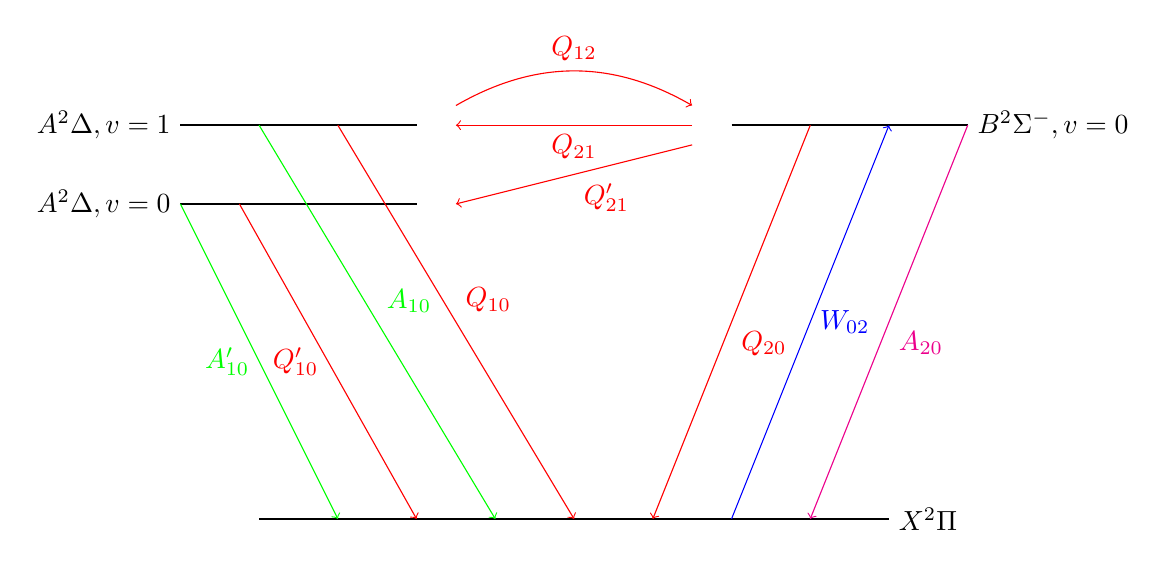
\begin{tikzpicture}

% Ground state
\draw [thick] ( 1, 0 ) -- ++( 8, 0 );
\node at ( 9, 0 ) [right] {\(X^2\Pi\)};

% First electronic states
\draw [thick] ( 0, 4 ) -- ++( 3, 0 );
\node at ( 0, 4 ) [left] {\(A^2\Delta, v = 0\)};
\draw [thick] ( 0, 5 ) -- ++( 3, 0 );
\node at ( 0, 5 ) [left] {\(A^2\Delta, v = 1\)};

% Second electronic state
\draw [thick] ( 7, 5 ) -- ++( 3, 0 );
\node at ( 10, 5 ) [right] {\(B^2\Sigma^-, v = 0\)};

% Transitions
\path [->, blue] ( 7, 0 ) edge node [right] {\(W_{02}\)} ++( 2, 5 );
\path [->, red] ( 8, 5 ) edge node [auto] {\(Q_{20}\)} ++( -2, -5 );
\path [->, magenta] ( 10, 5 ) edge node [auto] {\(A_{20}\)} ++( -2, -5 );

\path [->, red] ( 6.5, 5 ) edge node [auto] {\(Q_{21}\)} ++( -3, 0 );
\path [->, red] ( 6.5, 4.75 ) edge node [auto] {\(Q'_{21}\)} ++( -3, -0.75 );
\path [->, red] ( 3.5, 5.25 ) edge [bend left] node [above] {\(Q_{12}\)} ++( 3, 0 );

\path [->, red] ( 2, 5 ) edge node [auto] {\(Q_{10}\)} ++( 3, -5 );
\path [->, green] ( 1, 5 ) edge node [auto] {\(A_{10}\)} ++( 3, -5 );

\path [->, red] ( 0.75, 4 ) edge node [left] {\(Q'_{10}\)} ++( 2.25, -4 );
\path [->, green] ( 0, 4 ) edge node [left] {\(A'_{10}\)} ++( 2, -4 );

\end{tikzpicture}

\caption[Simplified CH energy level diagram]{A simplified model of the transitions between the energy levels in a CH system. Excitation (\textcolor{blue}{blue}) of ground state CH molecules to the upper electronic state is followed by several collisional energy transfer processes (\textcolor{red}{red}). A small portion of these molecules spontaneously emit a photon (\textcolor{green}{green}) and return to ground state. The spontaneous emission corresponding to resonant PLIF (\textcolor{magenta}{magenta}) is not collected.}

\label{fig:simplifiedEnergyLevels}

\end{figure}

